%%%%%%% TOOLS %%%%%%
\section{Libraries and technologies}
\label{libraries_and_technologies}

This section covers the different libraries and technologies used in the development of this thesis. First, the programming framework present in the project's progression is displayed, as well as the different third-party libraries and packages that has been employed in the software. Afterwards, the tools used for profiling and testing the code are analyzed and, finally, the hardware being used is presented and its main characteristics explained. 




	\subsection{ROS}
		\label{technologies_ros}
		\paragraph{ROS package: openni\_camera / freenect\_camera}\mbox{} \\

		These two ROS packages are the RGB-D sensors drivers. Both can be used just changing the name of the executable or launch file. This is due to the fact that both publish the same information in identic topics. 
		\\

		They are needed in order to connect the kinect to the computer. They transfom the raw output information of the computer into a ros message with the different images and point clouds. 
		\\

		In this project both have been used indistinctly.  

		\paragraph{ROS package: openni\_launch / freenect\_launch}\mbox{} \\

		These packages take as the input the information provided by the openni\_camera / freenect\_camera. They provide useful transformations and a launch file that executes nodelets with that information. This way, not only the raw image and point cloud from the kinect can be obtained but also the registered point cloud or the disparity image. 
		\\

		Both have been used in the code and they are the input to the pi\_tracker package which is explained in the next section. They are the input of the system as well, providing the point clouds and images that are later on segmented by this software. 


		\paragraph{ROS package: pi\_tracker}\mbox{} \\

		This package was developed by an MIT group. It publishes in the output a relation of the position and pose of each joint of the user. It is capable of recognizing more than one person at a time and to give the information about it. 
		\\

		The package easies the hand tracking algorithm since the input to it is the hand's position. It is very helpful to determine gestures made by the user due to the completeness of the information provided. 
		\\

		In order to publish the information about the joints, a custom message pi\_tracker/Skeleton is created. 

	\subsection{OpenCV}
		\label{technologies_opencv}
		\begin{itemize}
		\item\textbf{Segmentation of the ROI (Region Of Interest)\\ }

		This library allows to crop the original raw image coming
		from the RGB-D sensor. In this application, the region cropped is the one around the hand being used. More information about this operation can be found in the \ref{roi_segmenter_2d} section. 
		

		\item\textbf{ {Keypoints and descriptors extraction\\ }}

		 The OpenCV library implements multiple optimized state of the art algorithms. Among them, there are a number of descriptor extractors such as SIFT, SURF, ORB. This last one is being used in this project due to its open-sourceness, and robustness / speed relation. More information about the different algorithms implemented in OpenCV used to extract the descriptors can be found in the section \ref{features}.


		\item\textbf{ {Descriptors matching\\ } }

		There are many different matchers that might be used. In this project, a FlannBasedMatcher
		is being used for this purpose. 
		\end{itemize}

	\subsection{PCL}
		\label{technologies_pcl}
		The Point Cloud Library is used within the software to perform transformations in the input point clouds and to perform descriptor extraction and matching in this data. 
		\\

		More specifically, PCL is used in the following processes: 

		\begin{itemize}
			\item{\textbf{Segmentation of the ROI (Region Of Interest)\\ }}

			This library allows to crop the original raw point cloud coming from the RGB-D sensor. In this application, the region cropped is the one around the hand being used. More information about this operation can be found in the \ref{roi_segmenter_3d} section. 
			

			\item{\textbf{ Keypoints and descriptors extraction\\ }}

			 The PCL library implements multiple optimized state of the art algorithms. Among them, there are a number of descriptor extractors such as PFH, FPFH or LINEMOD. In this project, the PFH descriptor is used due to its speed. More information about the different 3D descriptors implemented in PCL can be found in the section \ref{3d_features}.


			\item {\textbf{Descriptors matching\\ }}

			There are different algorithms that allow to match the information provided by the descriptors, such as knn search or radius search. For further information about the type of matcher used in the present thesis, please visit the section \ref{learner_recognizer}
		\end{itemize}

	\subsection{Profiling}


	\subsection{Testing}
		\label{technologies_testing}
		In order to perform the code testing different technologies have been used that are specified in the following paragraphs. 
		\\


		\paragraph {Testing levels}\mbox{} \\

		There are different levels of testing that should be implemented in all software projects. Depending on the level of integration of the code within ROS, it is needed to code until one level or the other. 		\\

		If the software implements some ROS node that publishes or subscribes to a topic, then the three levels of testing are needed. If, on the contrary, it implements a ROS service, it is only necessary to test until the second level. A ROS-free library only needs the first level, the library unit testing. 
		\begin{itemize}

			\item{\textbf{First level: Library unit test}}\\

		A library unit test should test your code without ROS. If your code functionality is integrated directly with ROS functions, your library probably needs to be re-factored. 
		\\

		In the software developed the functionality of the nodes are separated from the ROS communication, allowing an easy unit testing. \\

		The library used to perform this unit testing is gtest. More information about that library may be found in the section \ref{gtest}.

			\item{\textbf{Second level: ROS node unit test\\}}

		In order to perform this testing level a library unit test and the rostest tool are needed. Here, the node unit tests start up the node and test its external API, the published and subscribed topics and services. 
		\\

		The rostest tool is explained in detail in the following \ref{rostest} section.

			\item{\textbf{Third level: ROS node integration / regression test}}\\

			This type of testing is directed to try the functioning of multiple nodes at the same time. 
			The debugging of a group of ROS nodes is similar to debugging mutithreaded code. \\

			In order to perform a third-level testing, both a unit testing library and the rostest tool are needed. 
		\end{itemize}

		\paragraph{gtest}\mbox{} \\

		\label{gtest}
		Gtest (Google Test) is used within the code to perform the first level testing. It is a testing framework for C++ that is cross-platform. It is based in the xUnit architecture and supports automatic test discovery, many different and user-defined assertions, death tests, fatal and non-fatal failures and various options for running the tests as well as XML test report generation. 
		\\

		Currently is included in ROS as a rosdep package that is installed automatically together with the Operating System. 


		\paragraph{rostest}\mbox{} \\

		\label{rostest}
		Rostest is an extention to roslaunch that allow launch files to be used as test fixtures. 
		In order to use it, new test nodes must be written that execute unit tests. 


	\subsection{Hardware}
		\label{technologies_hardware}

		The hardware needed in order to retrieve three-dimensional information is an RGB-D sensor compatible with the openni\_launch ROS package previously mentioned, and a computer running Linux. The information provided by this kind of device is more complete and makes the segmentation of the Region Of Interest easier. \\

		The sensor being used for the experiments presented in the following chapter is a Kinect of the Xbox 360. The reason of choosing this specific sensor is that it is cheaper than the other devices that include depth information. The main drawback with respect to other sensors such as the Asus Xtion PRO LIVE\cite{xtion} is that it needs a separate power plug to work, and also its size is bigger. 
		\\


		% In this section the main components and functioning principles of the Kinect are going to be presented. Most of them are common with the other RGB-D sensors but others such as the VGA camera are optional, for example in some PrimeSense\cite{PrimeSense} models. 

		\begin{figure}[h]
			\begin{center}
		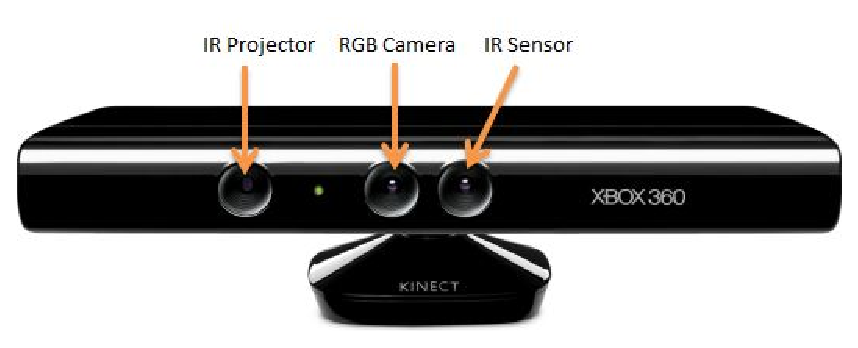
\includegraphics[scale=0.5]{img/kinect/kinect2.eps}
			\caption[Kinect Sensors]{Kinect sensors: depth sensor and VGA camera location.}
			\end{center}
		\end{figure}


		The parts that compose the Kinect sensor are the following: 

		\begin{itemize}
			\item{\textbf{VGA camera}}\\
			The camera contained by the kinect has a pixel resolution of 640x480 and a frame rate of 30 fps. It is used mainly to provide the output data with the RGB components for each point. 
			
			\item{\textbf{Depth sensor}\\
			The depth sensor consists on an infra-red projector combined with a monochrome CMOS sensor. This latter measures the time it takes the light to come back after being reflected on the objects. Knowing the speed of light it can be easily obtained the distance of the objects from the depth sensor. 

			\item{\textbf{Multi-array microphone}}\\
			This array of four microphones are included because the kinect was designed as a gaming device. They are not used for the three-dimensional world retrieving. 
			
			\item{\textbf{Motorized tilt}}\\
			This is another feature for games. It allows the kinect to follow the player's movements around the room. \cite{howkinectworks} The openni drivers do not allow to control this motor, but the freenect library does. Since the project is supposed to work on a robot with an independent head movement, this feature is not needed for the software and hence not being able to control the motor is not an issue. 
		\end{itemize}



		\begin{figure}[H]
			\begin{center}
			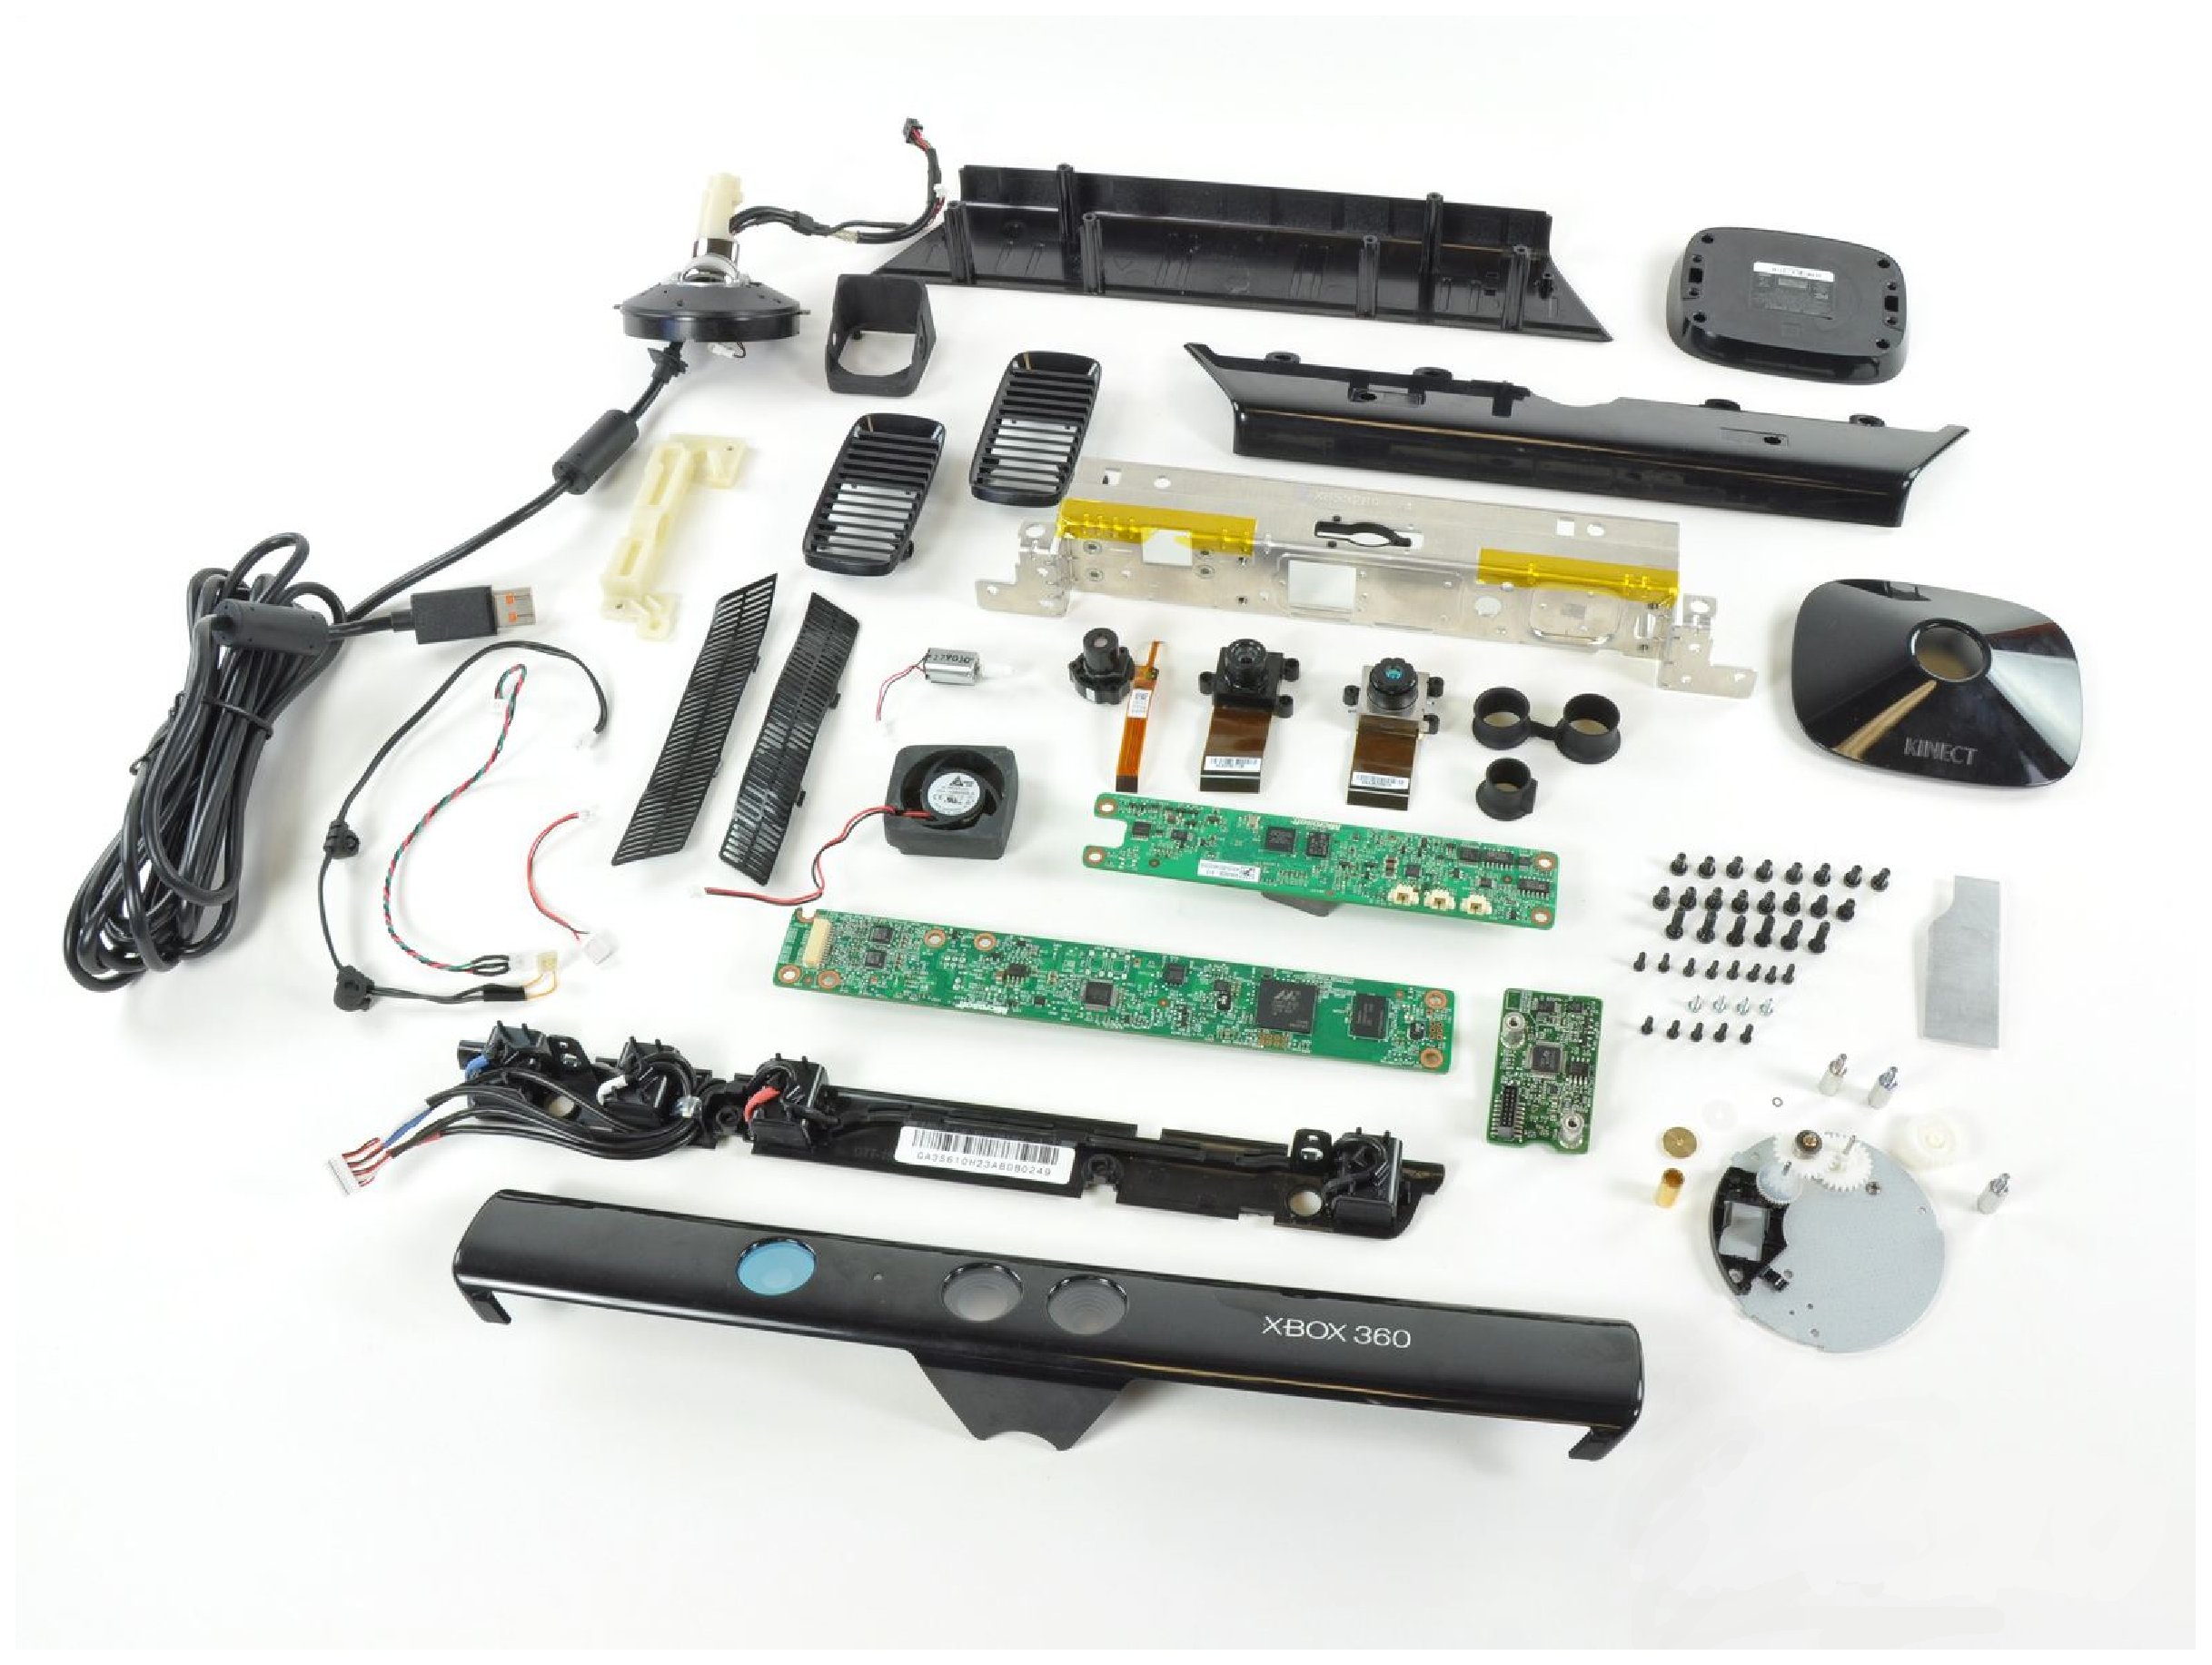
\includegraphics[scale=0.2]{img/kinect/kinect_parts.eps}
			\caption[Kinect Parts]{Kinect dismounted. Parts and components.}
			\end{center}
		\end{figure}


		The picture above shows the different parts that compose the kinect. In the middle of the image the depth sensor (IR emitter and receptor) and the VGA camera might be seen. Also, the boards with the signal conditioning circuit for the sensors are presented together with the different pieces of the structure of the sensor. The tilt motor is integrated within the support part and it is not visible. 